\section{Attitude Controller}
The angular response of the quadcopter constitutes a coupled behavior as the three Euler angles (\si{\phi}, \si{\theta} and  \si{\psi}) are affected by the four motor velocities. This makes it harder to utilize independent controllers for each angle. A state space approach is instead considered.   

In state space, the system behavior is represented by means of the linearized model equations. These show how the output and the states of the system evolve as a function of the current states values and the input applied to the system. \autoref{xDotDiffEq} and \autoref{yDiffEq} show the idea of state space representation.
%
\begin{flalign}
	\vec{\dot{x}}(t)&=f(\vec{x}(t),\vec{u}(t))
	\label{xDotDiffEq} 
\end{flalign}
\begin{flalign}
	\vec{y}(t)&=g(\vec{x}(t),\vec{u}(t)) 
	\label{yDiffEq} 
\end{flalign}
%
The description of the system can also be expressed in matrix form, giving \autoref{xDotLinear} and \autoref{yLinear}.
%
\begin{flalign}
	\vec{\dot{x}}(t)&=\vec{A} \  \vec{x}(t) + \vec{B} \  \vec{u}(t)
	\label{xDotLinear} 
\end{flalign}
\begin{flalign}
	\vec{y}(t)&=\vec{C} \  \vec{x}(t) + \vec{D} \  \vec{u}(t)
	\label{yLinear} 
\end{flalign}
%
\begin{where}
    \va{\vec{A}}{$=\frac{\partial}{\partial \vec{x} } \ f(\vec{x_o},\vec{u_o})$ \ \ is the $6 \times 6$ state feedback matrix}{}
    \va{\vec{B}}{$=\frac{\partial}{\partial \vec{u}} \ f(\vec{x_o},\vec{u_o})$ \ \ is the $6 \times 4$  input matrix}{}
    \va{\vec{C}}{$=\frac{\partial}{\partial \vec{x}} \ g(\vec{x_o},\vec{u_o})$ \ \ is the $3 \times 6$  output matrix}{}
    \va{\vec{D}}{$=\frac{\partial}{\partial \vec{u}} \ g(\vec{x_o},\vec{u_o})$ \ \ is the $3 \times 4$  feedforward matrix}{}
\end{where}

This state space description can be seen also in the form of a block diagram like the one shown in \autoref{SSBlocks}.
%
\begin{figure}[H]
	\begin{tikzpicture}[ auto,
                       thick,                         %<--setting line style
                       node distance=1.5cm,             %<--setting default node distance
                       scale=1,                     %<--|these two scale the whole thing
                       every node/.style={scale=1}, %<  |(always change both)
                       >=triangle 45 ]                %<--sets the arrowtype
    
    \draw%-----------------------------------------------------------------------------------------
    	%Drawing Input/Output:
    	node[shape=coordinate][](input1) at (0,0){}
    	node[shape=coordinate][](output1) at (9.5,0){}
     	%Drawing the Equation Blocks:   	
      	node(A) at (4.5,-1.5) [block] {A} 
     	node(B) at (1.5,0) [block] {B}
     	node(C) at (6.5,0) [block] {C}
      	node(D) at (4.5,1.5) [block] {D}  
	    node(int) at (4.5,0) [block] {\si{\int}}  
    	%Drawing the Sumation Blocks:	    	 	
    	node(sum1) [sum, right of = B] {\si{\sum}}
    	node(sum2) [sum, right of = C] {\si{\sum}}
    	%Drawing the Feedback/Feedforward Nodes:    	
    	node[shape=coordinate][](FeedforwardNode) at (0.75,0){}
    	node[shape=coordinate][](FeedbackNode) at (5.5,0){}  	
    	     
    ;%---------------------------------------------------------------------------------------------
   
    %Joining the Blocks
  	\draw[->](input1) -- node {u}(B);
  	\draw[->](B) -- node {}(sum1);
  	\draw[->](sum1) -- node {\si{\dot x}}(int);  	
  	\draw[->](int) -- node {x}(C);
  	\draw[->](C) -- node {}(sum2);  	
  	\draw[->](sum2) -- node {y}(output1);
  	
  	\draw[->](FeedforwardNode) |- node{} (D);
  	\draw[->](D) -| node{} (sum2);

  	\draw[-] (FeedbackNode) |- (A);
  	\draw[->] (A)   -| (sum1);

    %Drawing node(s) with \textbullet
    \draw%--------------------------------------------------------------
      node at (input1)  [shift={(-0.08, -0.02 )}] {\large \textbullet}
    	% node at (output1) [shift={( 0.008, -0.02 )}] {\textbullet}
    ;%------------------------------------------------------------------
  \end{tikzpicture}
	\centering
	\caption{Block diagram of the state space representation of the system.}
	\label{SSBlocks}
\end{figure}\vspace{-18pt}
%
As the orientation of the quadcopter is to be controlled and the differential equations that describe the behavior include the angular accelerations, the state vector is chosen to be formed by the angles and the angular velocities. The input vector contains the four motor velocities and the output is constructed by the angles \si{\phi}, \si{\theta}, \si{\psi}. These vectors can be seen in \autoref{uVector}.\\
\begin{minipage}{0.32\linewidth}
	\begin{flalign}
		\vec{x}(t) = 
		\begin{bmatrix}
			\phi \\
			\theta \\ 
			\psi \\
			\dot{\phi} \\
			\dot{\theta} \\
			\dot{\psi} \\
		\end{bmatrix}	\nonumber
		\label{xVector}
	\end{flalign}  
\end{minipage}\hfill
%\hspace{0.03\linewidth}
\begin{minipage}{0.32\linewidth}
	\begin{flalign}
		\vec{y}(t) = 
		\begin{bmatrix}
			\phi \\
			\theta \\ 
			\psi \\
		\end{bmatrix}	\nonumber
		\label{yVector}
	\end{flalign}
\end{minipage}\hfill
%\hspace{0.03\linewidth}
\begin{minipage}{0.32\linewidth}
	\begin{flalign}
		\vec{u}(t)= 
		\begin{bmatrix}
			\omega_1 \\
			\omega_2 \\
			\omega_3 \\
			\omega_4 \\
		\end{bmatrix}\textsl{}
		\label{uVector}
	\end{flalign}
\end{minipage}\hfill
\\
The specific matrices for the description of the angular behavior are obtained from the linearized equations of the system (\autoref{eqAngleLin1} and \ref{eqAngleLin2}) and they are showed embedded in the state space representation in \autoref{xDotSS} and \autoref{ySS}.

\begin{flalign}   \label{xDotSS}
	\vec{\dot{x}}(t) &=
	\begin{bmatrix}
		\ 0 & 0 & 0 & 1 & 0 & 0     \ \ \ \\ 
		\ 0 & 0 & 0 & 0 & 1 & 0     \ \ \ \\ 
		\ 0 & 0 & 0 & 0 & 0 & 1     \ \ \ \\
		\ 0 & 0 & 0 & 0 & 0 & 0     \ \ \ \\ 
		\ 0 & 0 & 0 & 0 & 0 & 0     \ \ \ \\ 
		\ 0 & 0 & 0 & 0 & 0 & 0     \ \ \ 		
	\end{bmatrix}
	\vec{x}(t) +
	\begin{bmatrix}
		\ 0 & 0 & 0 & 0      \ \ \ \\ 
		\ 0 & 0 & 0 & 0      \ \ \ \\ 
		\ 0 & 0 & 0 & 0      \ \ \ \\
		\ 0 & \si{-\frac{2 \  k_{th} \  L \  \overline{\omega}_2}{J_x}} & 0 & \si{\frac{2 \  k_{th} \  L \  \overline{\omega}_4}{J_x}}      \ \ \ \\ 
		\ \si{\frac{2 \  k_{th} \  L \  \overline{\omega}_1}{J_y}} & 0 & \si{-\frac{2 \  k_{th} \  L \  \overline{\omega}_3}{J_y}} & 0      \ \ \ \\ 
		\ \frac{2 \  k_d \  {\overline{\omega}_1}}{J_z} & - \frac{2 \  k_d \  {\overline{\omega}_2}}{J_z} & \frac{2 \  k_d \  {\overline{\omega}_3}}{J_z} & - \frac{2 \  k_d \  {\overline{\omega}_4}}{J_z}      \ \ \ 		
	\end{bmatrix}
	\vec{u}(t)
\end{flalign}
\begin{flalign} \label{ySS}
	\vec{y}(t) &=	 
	\begin{bmatrix}
		\ 1 & 0 & 0 & 0 & 0 & 0     \ \ \ \\ 
		\ 0 & 1 & 0 & 0 & 0 & 0     \ \ \ \\ 
		\ 0 & 0 & 1 & 0 & 0 & 0     \ \ \ 		
	\end{bmatrix}
	\vec{x}(t)
\end{flalign}


The dynamics of the system can be analyzed by looking at the system matrix A. The eigenvalues of this matrix represent the location of the open loop poles of the system. In this case, the system shows 6 poles located in zero, which means that the system is marginally stable. In order to place those poles at a better location state feedback is used together with an integral action to be able to set a desired reference for the angles that is different from zero. 

As the output is formed by the the three angles, these are the only measured states in the system. For doing the state feedback, the angular velocities are also needed. The way of obtaining it i chosen to be a reduce order observer even though when using the Vicon system, the angular velocities could be estimated with a numerical differentiation procedure. The observer is more convenient in case of using on board sensors and by using it, that possibility is kept open.

This way of approaching the control of the system is simplified by the possibility of designing the state feedback and integral controller and the observer independently. This holds due to the separation principle.

Before designing the controller and the observer, it is advisable to check the controllability and observability of the system. For doing so, the matrices shown in \autoref{controlabilityandobservability} are used.\\
\begin{minipage}{0.45\linewidth}
\begin{flalign}
\vec{{\mathcal C}} = 
\begin{bmatrix}
\vec{B}&\vec{A}\vec{B}&\vec{A^2}\vec{B}&\vec{A^3}\vec{B}&\vec{A^4}\vec{B}&\vec{A^5}\vec{B} \\	
\end{bmatrix}\nonumber 
\end{flalign}
\end{minipage}\hfill
%\hspace{0.03\linewidth}
\begin{minipage}{0.45\linewidth}
\begin{flalign}
\vec{{\mathcal O}} = 
\begin{bmatrix}
\vec{C} \\
\vec{C}\vec{A} \\
\vec{C}\vec{A}^2 \\
\vec{C}\vec{A}^3 \\
\vec{C}\vec{A}^4 \\
\vec{C}\vec{A}^5 \\		
\end{bmatrix}					\label{controlabilityandobservability} 									
\end{flalign}
\end{minipage}\hfill

The rank of these matrices is 6, that is, the number of states. This makes the system both controllable and observable. The precise value of the matrices can be seen in \autoref{app:matricesSS}.

The block diagram showing the system overview of the attitude controller is showed in \autoref{attitudecontrollerdiagram}, in which the state feedback, the integral control and the observer can be seen.
\begin{figure}[H]
	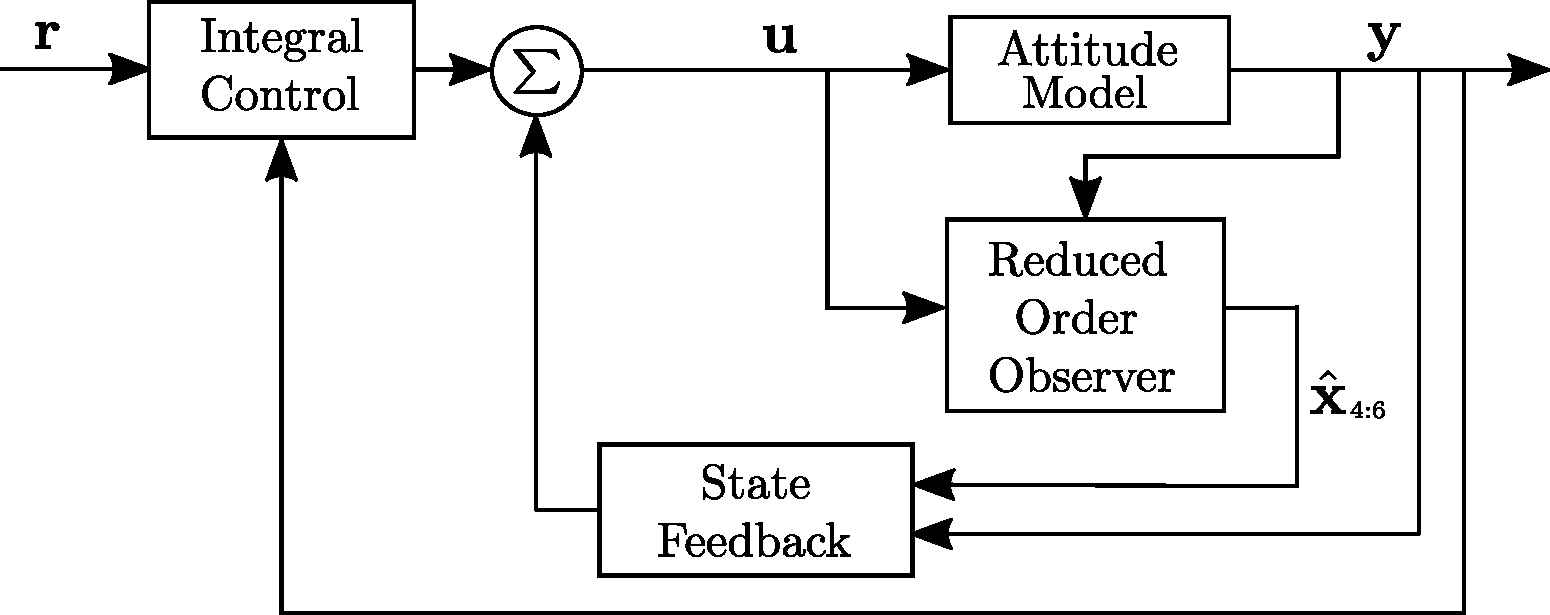
\includegraphics[scale=.5]{figures/AttitudeControlDiagram}
	\centering
	\caption{Control structure for the system, including the state feedback, the integral control and the reduced order observer.}
	\label{attitudecontrollerdiagram}
\end{figure}


